
\label{chapter:unit_tests}

In addition to the \maestro\ science problems, which use the full
capabilities of \maestro, there are a number of unit tests that
exercise only specific components of the \maestro\ solvers.  These
tests have their own drivers (a custom {\tt varden.f90}) that
initialize only the data needed for the specific test and call
specific \maestro\ routines directly.


\section {\tt test\_advect}

  This test initializes a Gaussian density field (no other scalar
  quantities are used) and a uniform velocity field in any one of the
  coordinate directions.  The Gaussian profile is advected through
  the period domain exactly once and the error in the density profile
  (L2 norm) is computed.  The driver for this problem does this 
  for every dimension twice (once with a positive velocity and once
  with a negative velocity).  After all coordinate directions are 
  tested, the norms are compared to ensure that the error does
  not show any directional bias.


\section {\tt test\_average} 

  This test initializes a 1D radial base state quantity with a
  Gaussian distribution, maps it into the 3D domain (assuming a
  spherical geometry) using the routines provided by the {\tt
    fill\_3d\_module} module, and then calls {\tt average} to put it
  back onto a 1D radial array.  This way we test the accuracy of our
  procedure to map between the 1D radial and 3D Cartesian states.
  The output from this test was described in detail in
  \cite{multilevel}.


\section {\tt test\_basestate} 

  This test initializes the base state to contain a hydrostatic
  model and then evolves the state with heating to watch the 
  hydrostatic adjustment of the atmosphere.  In particular,
  the base state velocity, $w_0$, is computed in response to 
  the heating and this is used to advect the base state density
  and compute the new pressure, $p_0$.  An early version of 
  this routine was used for the plane-parallel expansion test
  in \cite{lowMach2}.  This version of the test was also shown
  for a spherical, self-gravitating star in \cite{multilevel}.

  
\section {\tt test\_diffusion}

  This test initializes a Gaussian temperature profile and calls
  the thermal diffusion routines in \maestro\ to evolve the state 
  considering only diffusion.  The driver estimates a timestep
  based on the explicit thermal diffusion timescale and loops
  over calls to the thermal diffusion solver.  A Gaussian remains
  Gaussian when diffusing, so an explicit error can be computed
  by comparing to the analytic solution.  This test is 
  described in \cite{xrb}.


\section {\tt test\_eos}

  This test sets up a 3-d cube with $\rho$ varying on one axis, $T$ on
  another, and the composition on the third.  The EOS is then called
  in every zone, doing $(\rho, T) \rightarrow  p, h, s, e$  and stores those
  quantities.  Then it does each of the different EOS types to recover
  either $T$ or $\rho$ (depending on the type), and stores the new $T$ (or
  $\rho$) and the relative error with the original value.  A plotfile is
  stored holding the results and errors.  This allows us to determine
  whether the EOS inversion routines are working right.


\section {\tt test\_particles}

  This test exercises the particle advection routine.  A simple
  circular velocity field, with the magnitude increasing with radius
  from the center is initialized.  A number of particles are then
  initialized at various radii from the center and they are advected
  for one period.  The particle paths should be perfect circles, and
  the final particle position should overlap with the initial
  position.

  Particle data is stored separately from the fluid data.  Instead
  of being part of the plotfiles, the particle data is outputted
  each timestep into files named {\tt timestamp\_*}, where 
  the number indicates which processor did the writing.  These
  particle files can be processed and the particle data plotted
  using the python routines in {\tt data\_processing/python/}.

  The output from this test can be visualized with the script {\tt
  plot.py} in the test directory.  The output shows the particle
  paths (see figure~\ref{fig:unit:particles}).

\begin{figure}[t] 
\centering
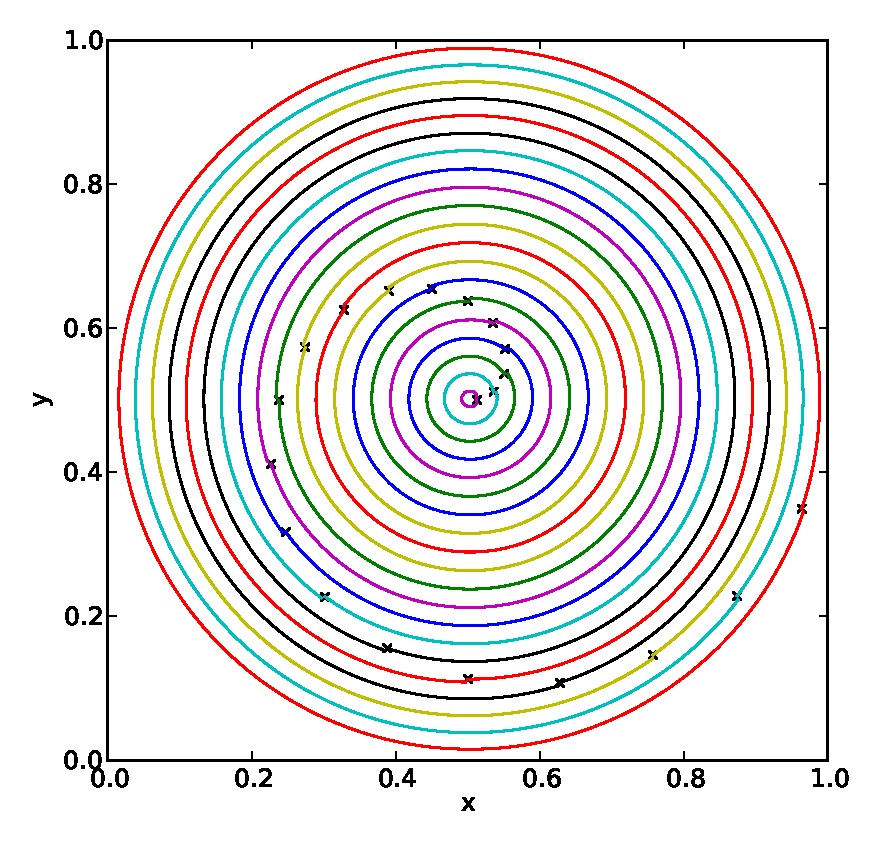
\includegraphics[width=4in]{\unitfigpath/particle_paths} 
%
\caption[Particle paths for the {\tt test\_particles} problem]{\label{fig:unit:particles}
  Particle paths for the {\tt test\_particles} problem.  The initial
  position of the particles is marked with an $\times$.}
\end{figure}


\section {\tt test\_projection}

  This tests the hgprojection routine in 2-d.  A divergence-free
  velocity field is initialized and then ``polluted'' by adding the
  gradient of a scalar.  The form of the scalar differs depending on
  the boundary conditions (wall and periodic are supported currently).
  Finally, the hgproject routine is called to recover the initial
  divergence-free field.  




